% Document history:
%  1.0 - Original version by Will
%  1.1 - Updated version including new problems
%
\documentclass[11pt,a4paper]{scrartcl}
\usepackage{graphicx}
\usepackage{acronym}
\usepackage{fancyhdr}

\setlength{\parskip}{1.5ex\relax}

\setlength{\fboxsep}{2mm} \setlength{\fboxrule}{0.8pt}  %% default=0.4

% Problems with this function:
%    1. Breaks headings as they loose the \noindent
\newcommand{\funbox}[1]{\vbox{\vspace{0.2cm}\fbox{\large\texttt{#1}}\vspace{0.2cm}}}
\def\cpp{C$++\;$}
\def\main{\texttt{main()}$\;$}
\def\intmain{\texttt{int main()}$\;$}
\def\void{\texttt{void}$\;$}
\def\public{\texttt{public}$\;$}
\def\private{\texttt{private}$\;$}
\def\protected{\texttt{protected}$\;$}

\begin{document}
\title{\cpp Programming for Physicists}
\author{W. H. Bell}
\date{
\copyright 2009
}

\maketitle
\hrule
\vspace{0.2cm}
\begin{abstract}

The \cpp language is introduced through a series of example programs
relevant to high energy physicists.  The course introduces basic
syntax, object orientated programming, the Standard Template Library,
interfacing with FORTRAN and high energy packages HepMC, HepPDT,
and ROOT.  Programming skills and design proccesses are introduced
within the discussion of the example programs.  The understanding of
\cpp programming concepts is tested though set problems, for which
associated solutions are provided.

\end{abstract}
\vspace{0.2cm}
\hrule

\clearpage
\newpage

\tableofcontents

\clearpage
\newpage

\pagestyle{fancy}

\section{Introduction}

\cpp is used for a large number of applications within industry and
Particle Physics research.  The language provides a large amount of
functionality and is still being extended.  This course focuses on
core aspects of \cpp and expects the reader will consult reading
materials to extend this introduction.  The recommended reference
materials for this course are:
%
\begin{itemize}
\item ``Ivor Horton's Beginning C++'', Ivor Horton, Apress, ISBN 1590592271
\item ``The C++ Programming Language'', Bjarne Stroustrup, Addison-Wesley, 1997
\end{itemize}
%
The course is largely based on the ANSI standard and should therefore
compile with any standard \cpp compiler.  Since most Particle Physics
applications are build on LINUX or OSX, instructions to compile on
LINUX or OSX are provided.

%%%%%%%%%%%%%%%%%%%%%%%%%%%%%%%%%%%%%%%%%%%%%%%%%%%%%%%%%%%%%%%%%%%%%%%%%%%%

\section{\cpp Syntax \label{section:cppsyntax}}
This section discusses basic data types and simple \cpp syntax which are largely common between \cpp, C and JAVA.

%-----------------------------------------------------------------------------

\subsection{A First Program}

Programming languages are commonly introduced by writing a program to
print a string to the standard output.  The standard output is
normally visible on the terminal window or screen.  Using just \cpp
syntax this is simply demonstrated by example~1:

\begin{verbatim}
/* W. H. Bell
** A very simple C++ program to print one line to the standard out
*/

#include <iostream>

using namespace std;

int main() {
  cout << "In the beginning..." << endl;
  return 0;
}
\end{verbatim}

The execution of every program starts from a \main function.  From
this function other functions can be called.  The return type of \main
is given by the \texttt{int} prefix.  Within the LINUX/UNIX
environment the operating system expects a program to return an exit
condition.  The value of the return statement from the \main function
is collected by the operating system and is available to a user to
query.  For example, at a LINUX shell prompt \texttt{`]\$'} one could type:

\begin{verbatim}
]$ ./InTheBeginning.exe 
In the beginning...

]$ echo $?
0
\end{verbatim}
%$
where \texttt{\$?} contains the return value of the last command.

The contents of the first example's \main function are delimited by
the brackets~\texttt{\{~\}}, which represent a compound statement.
Inside this compound statement there may be several statements each
terminated by a `\texttt{;}' character, together with other compound
statements.  In this example the \main function only contains two
statements: one to print a string to the standard output and one to
return the exit value to the operating system.  The first of these
statements prints a string to the screen by calling the standard
output stream function \texttt{cout} with the insertion operators
\texttt{<<}.  This operator can be used to concatenate strings.  In
the given example the end of line character \texttt{endl}, is appended
to the string \texttt{"In the beginning..."}.  At the top of the
example the declaration of the \texttt{cout} function is included by
including the header file \texttt{iostream}.  When this program is
compiled the compiler reads the pre-declaration of \texttt{cout} from
the header file and leaves a call in the machine code to be resolved
at link time.

Finally in this first program one of the two comment styles is
introduced.  Comments in \cpp can be entered in two ways: 
\texttt{/* */} can be used to surround the comment area or 
\texttt{//} can be used at the start of each comment line.

%-----------------------------------------------------------------------------

\subsection{Loops, Conditional Statements and Functions}
\paragraph{Functions}
The syntax of loops, conditional statements and functions are
demonstrated by example~2.  This example contains an \intmain function: the same as seen within the previous example.  Within this \main function three functions are called:
\texttt{numFingers}, \texttt{pickColour}, and
\texttt{quitTime}.  Each function is pre-declared before the \main
function.  Each pre-declaration is a statement where the return type,
and input parameter types must be given.  The \void type simply means that
no input parameter or return value is expected.  All functions must be
either predeclared or declared before they are used.  There are three
pre-declaration statements before the \main function:
\begin{verbatim}
void numFingers(void);
void pickColour(void);
bool quitTime(void);
\end{verbatim}
where the implementation of these functions is given after the \main
function.  Following the same syntax as the \main function the
implementation of each of these three functions has a return type, a
series of input types, and a compound statement enclosing the function
contents.  If any input parameters are present then their names must
be given in functions implementation.  When a function is called the
input variables are allocated in memory and are initialised with the
values passed into the function.  If the implementation is not given in
either the code to be compiled, or libraries to be linked against, a linker
error will result.

\paragraph{Conditional Statements}
Conditional logic is essential for the control of both loops and
selection statements.  Most common of the the selection statements
are: \texttt{if},~\texttt{if~else},~\texttt{else} and \texttt{switch}
statements.\footnote{There are other ways of constructing conditional
statements but they are not covered in this course.}

Example~2 provides a demonstration of the syntax of
\texttt{if},~\texttt{if~else},~\texttt{else} constructs:
\texttt{if},~\texttt{if~else},~\texttt{else} syntax is implemented
within the \texttt{numFingers} and \texttt{quitTime} functions of this
example.  The evaluation of an \texttt{if} statement follows simply:
if the logic within in the \texttt{()} brackets is true then the
following compound statement is executed.
\texttt{if},~\texttt{if~else},~\texttt{else} statements operate
sequentially such that each piece of logic is tested in turn.  If all
the logic tests fail then the statement following \texttt{else} is
executed.

In some cases where simple sorting is needed a \texttt{switch}
statement is a better choice than a long
\texttt{if},~\texttt{if~else}...~\texttt{else} statement: it provides a simple construct which executes quickly.  An example
\texttt{switch} statement is given in the \texttt{pickColour} function
of example~2.  While faster than an
\texttt{if},~\texttt{if~else},~\texttt{else} statement in some cases a
\texttt{switch} statement is limited to the usage
of simple cases and therefore the logic allowed can be somewhat
restrictive.

\paragraph{Loops}
Several types of loops are available to \cpp programmers: there are
\texttt{while}, \texttt{do~while} and \texttt{for} loops.  Each of
these loops continue to loop while a condition is true.  All the logic
available within an \texttt{if} conditional statement is also
available within the conditional test of a loop statement.  Instances
of these loop types can be found within many of the examples provided
in this course.  To begin with a simple example of a \texttt{do~while}
loop can be found in the \main function of example~2.  This loop
continues while the boolean evaluated within the \texttt{while( );} is
true.  This remains true until the function \texttt{quitTime} returns
a true, where: \texttt{while} loop tests on NOT \texttt{quitTime} return value.

%-----------------------------------------------------------------------------

\subsection{Pointers and Arrays \label{section:pointersarrays}}
Many languages e.g. Fortran and Java use pointers implicitly.  In
\cpp pointers are used explicitly.  This section introduces the
concept of a pointer and demonstrates two basic implementations.

Pointers are called pointers because they point to a memory address.
A pointer can be used to access the memory address to which it points
or the value contained within the memory address.  Example~3
introduces pointers.  Looking at example~3 there are two distinct
parts to the program: the call to the function \texttt{fun} and the
indexing of array \texttt{v[]}.

\paragraph{Functions and Pointers}

The function \texttt{fun} is declared as 
\begin{verbatim}void fun(int, int *);\end{verbatim}
with input parameter types \texttt{int} and \texttt{int *}.  The
second input parameter is a pointer.  When the function is called the
memory address of \texttt{p}, \texttt{\&p} is assigned to the pointer
declared in \texttt{fun}.  The importance of using a pointer in this
fashion can be seen from running the program.  After calling
\texttt{fun} the value of \texttt{np} is the value which it contained
before the function call, while the value contained in \texttt{p} is
the value assigned via the pointer in
\texttt{fun}.  Stepping through the program this can be explained.
Both \texttt{np} and \texttt{p} are initialised with the value one.
\begin{verbatim}int np = 1, p = 1;\end{verbatim}
At the point of initialisation an \texttt{int} sized block of memory
is allocated to \texttt{np} and \texttt{p}.  Then the function
\texttt{fun} is called with the value of \texttt{np} (default in \cpp) and the
address of \texttt{p}.  Within the function \texttt{fun} a new block
of memory is allocated for the local variable \texttt{np} distinct
from the variable contained in the \main function.  This memory is
given the value from the parameter \texttt{np} contained within
\main.  The value 2 is assigned to the local variable \texttt{np}
and as the function exits, the memory of the local variable \texttt{np}
is deleted.  Therefore the value is never set within the \main
function.

Unlike \texttt{np} the value of the variable \texttt{p} declared within
the \main is set by using a pointer.  The pointer is initialised with the
memory address of the variable \texttt{p} contained within the \main
function.  Then the memory address pointed to by the pointer
\texttt{*p} is assigned the value 2.  Therefore when returning to the
\main function the value contained in the memory of \texttt{p} is
still 2.

\paragraph{Arrays and Pointers}

An array of type {\it t} is a series of memory blocks of which the
size is fixed by the type {\it t}.  Each element of the array behaves
as a variable of type {\it t}.

In example~3 an array \texttt{v} is declared with four elements:
\begin{verbatim}int v[] = {1,2,3,4};\end{verbatim}
This code is equivalent in function to:
\begin{verbatim}
int v[4];
for(int i=0;i<4;i++) v[i]=i;
\end{verbatim}
The size of the array within example~3 is determined by the number of
elements within the brackets \texttt{\{\}}.  After the array has been
declared the address of the first element is assigned to the pointer
\texttt{*pv}.  It is important to note that the assignment of an
address to a pointer at declaration has different syntax to any
following assignment or operation on the pointers address in general.
The declaration of \texttt{*pv} and its assignment of the address of
the first element of the array \texttt{v} could alternatively be
written as:
\begin{verbatim}
int *pv;
pv=&v[0];
\end{verbatim}
Once the pointer has been assigned the memory address of the first
element of the array \texttt{v} it can be used to access the
elements as demonstrated in the example.

%-----------------------------------------------------------------------------

\subsection{Basic File Streams}

File stream functionality is included within a program by including
the \texttt{fstream} header file.  Example~5 demonstrates some input
and output stream functionality.  The program reads some text from the
command line.  Then this text is used to determine the file name and
if the file is to be written or read.  Depending on the command line
input the \main function calls one of two functions \texttt{fileWrite}
or \texttt{fileRead}.  The file \texttt{main.c} does not contain the
implementation of \texttt{fileWrite} and \texttt{fileRead}, but
includes the header file \texttt{FileIO.hh}: containing their
pre-declaration.  This program cannot be linked into an executable
without the implementation of the \texttt{fileWrite}
and \texttt{fileRead} functions being made available at link time.
\texttt{fileWrite} and \texttt{fileRead} are in fact implemented in
the file \texttt{FileIO.cc}, which is compiled and then linked with
\texttt{main.o}.

The function \texttt{fileWrite} opens an output stream, using the file
name supplied.
\begin{verbatim}
ofstream file(filename);
\end{verbatim}
Then this file output stream is used in exactly the same way as the
standard output stream in the previous examples.  Finally at the end of the
file operation the stream is closed.
\begin{verbatim}
file.close();
\end{verbatim}
Closing the file output stream is essential to flush the data stored
in the output memory to the file.  (Flushing is not always implicit to
a file stream being closed.)

The function \texttt{fileRead} uses an input file stream to read the
data from the specified file name.  It is initialised in the similar
way to the file output stream.
\begin{verbatim}
ifstream file(filename);
\end{verbatim}
If for some reason the file opening operation fails the file input
stream variable \texttt{file} will be assigned 0.  Any integer number
that is not 0 is considered logically as true.  0 is considered
logically as false and hence the usage of the \texttt{if} statement.
\begin{verbatim}
if(!file) {
  cerr << "Error: could not open " << filename << endl;
}
\end{verbatim}
The design of example~5 is illustrated in figure~\ref{figure:ex5_flowchart} and~\ref{figure:ex5_pseudocode}.

\begin{figure}[h!!]
\begin{center}
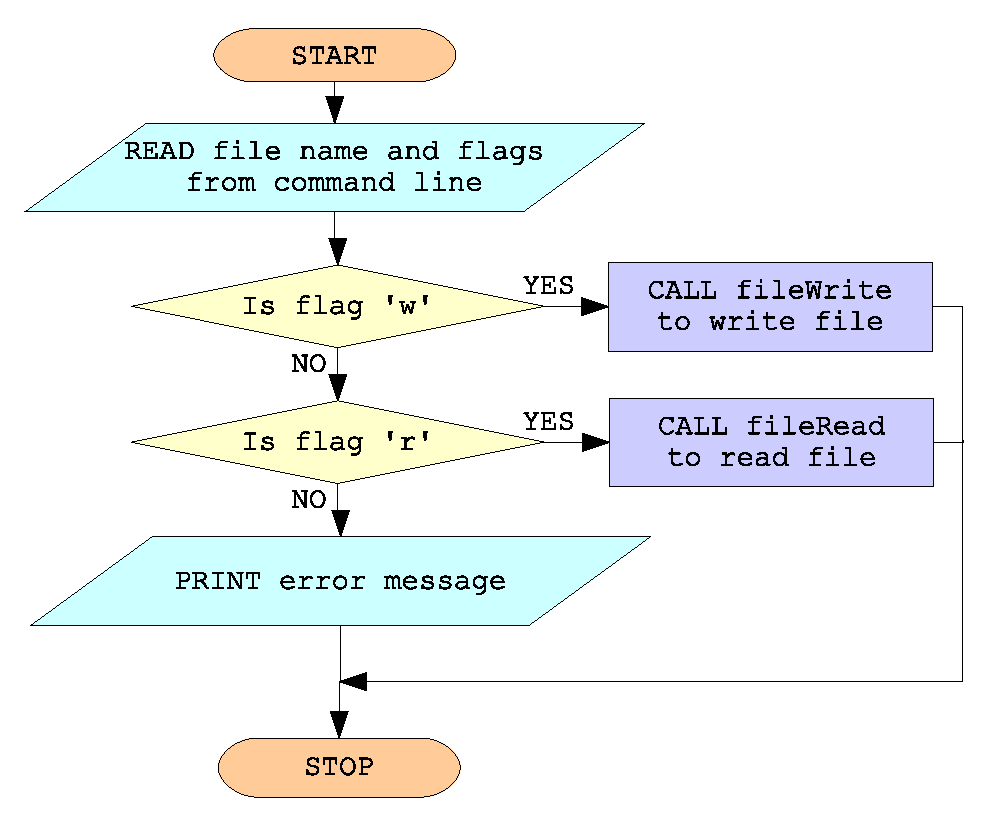
\includegraphics[height=9cm]{figures/flowchart.eps}
\caption{A flowchart describing example~5 in general terms.
\label{figure:ex5_flowchart}}
\end{center}
\end{figure}

\newsavebox{\fmbox}
\begin{lrbox}{\fmbox}
\begin{minipage}{13cm}
\begin{verbatim}
main() 
  Get command line arguments:
    Require 2 or 3 arguments: 
      First additional argument - file name
      Second additional argument - read/write flag.
  Use the value of the read/write flag to call either 
  fileRead() or fileWrite().

fileRead()
  Open an input stream.
  Read the contents of the file until the EOF.
    Stream each character number into a integer.
    Print these integers in the format of the file.
  Close the input stream.

fileWrite()
  Open an output stream.
  Loop from the numbers 1 to 20.
    Write out each number followed by a space to the 
    active file stream.
    After each fifth number is written append a new line.
  Close the output stream.
\end{verbatim}
\end{minipage}\end{lrbox}

\begin{figure}[h!!]
\begin{center}
\fbox{\usebox{\fmbox}}
\end{center}
\caption{Example 5 in pseudocode.
\label{figure:ex5_pseudocode}}
\end{figure}

\clearpage
\newpage

%=============================================================================

\subsection{Problems}
\paragraph{Reading a Configuration File}

Write a program to read in the table of particle data contained in the
file \texttt{problem\_01/particle.dat}.  Read each column of data into a
separate two dimensional \texttt{char} array.  Then use these arrays
to print each column of \texttt{particle.dat} to the screen.

\begin{enumerate}
\item Start by opening a file as demonstrated in example~5.
Then use the input stream function \texttt{getline}\footnote{The first
argument is a character array, the second argument is the length of
the array and the return value is the length of the string} to read
lines from the file.
\begin{verbatim}
  char str[MAX_LINE_LENGTH];
  int lineLength;
  ...
  ...
    while(!file.eof()) {
      file.getline(str,MAX_LINE_LENGTH);
      lineLength = strlen(str);
\end{verbatim}
\item Skip any lines that begin with a comment character:
\begin{verbatim}
      if(str[0]!="#") { // If character isn't # 
      ...
      }
\end{verbatim}
\item And parse each column of the file, skipping spaces as necessary.
\end{enumerate}

\noindent The function \texttt{strcpy} from the \texttt{cstring}
header file should be helpful for copying a section of a \texttt{C}
string.  The 
string terminator `\texttt{$\backslash$0}' can be used to terminate a
\texttt{C} string: where the maximum length is determined by the size
of the character array but the minimum length is set by the position
of the string terminator within the array.

\paragraph{File Encryption} 
Write a program to `encrypt' text files by using a binary mask e.g.:
\begin{verbatim}
  int mask = 0xA3;  // A number less than 255
  char c;           // The character to be read and encrypted/decrypted.
\end{verbatim}

\begin{itemize}
\item Read one byte from the standard input, encrypt
it and print the result to the standard output, e.g.:
\begin{verbatim}
  while((c=std::cin.get())!=EOF) { // Get character until end of file.
    //Replace this line with a bitwise operation.
    std::cout << c; //output character.
  }  
\end{verbatim}

\item Use one bitwise exclusive \texttt{OR} operation to encrypt and another to
decrypt e.g.:\\ 
\texttt{a = a \^{$\:$} mask}\\
(Two exclusive \texttt{OR} operations cancel.) 

\item Having written the encryption program, check the executable works by
using the command line syntax:
\begin{verbatim}
encrypt.exe < inputfile > outputfile
\end{verbatim}
\end{itemize}

\paragraph{EPS File Extraction}
Many postscript files contain embedded eps files which can be
extracted and saved in a separate file.  Write a program to parse the
file \texttt{problem\_03/document.ps}, saving any instances of
\begin{verbatim}
%%BeginDocument: 
...
%%EndDocument
\end{verbatim}
to files of appropriate names.

\begin{enumerate}
\item Open an input file stream:
\begin{verbatim}
std::ifstream file(argv[1]);
                                                                             
  if(!file) {
    std::cerr << "Error: could not open " << argv[1] << std::endl;
  }
  else {
   ...
  }
\end{verbatim}

\item Read single lines from \texttt{problem\_03/document.ps}:
\begin{verbatim}
    while(!file.eof()) { // While not end of file
      file.getline(line,MAX_LINE_LENGTH);  // Read one line.
      ...
    }
\end{verbatim}

\item Use the functions \texttt{strstr} and \texttt{strlen} from
\texttt{cstring} to catch included documents:
\begin{verbatim}
  char beginDocument[]="%%BeginDocument: "; // declare C string
  char endDocument[]="%%EndDocument"; // declare C string
  ...
  ... 
      if((filename=strstr(line,beginDocument))!=NULL) { // If begin document
        filename += strlen(beginDocument);  // File name follows %%BeginDocument:
        outputFile =  new std::ofstream(filename); // Open output file
      }
\end{verbatim}
where \texttt{filename} is of type \texttt{char*}.

\item Save a copy of the information between and including the
\texttt{\%\%BeginDocument} and \texttt{\%\%EndDocument} statements to
a separate file.
\end{enumerate}

%%%%%%%%%%%%%%%%%%%%%%%%%%%%%%%%%%%%%%%%%%%%%%%%%%%%%%%%%%%%%%%%%%%%%%%%%%%%%%

\section{Object Orientated Programming \label{section:ooprog}}

For many years developers have worked with languages such as FORTRAN
and \texttt{C}.  These languages allow developers to write functions
and complicated data blocks.  While suitable for many applications
large programs written with these languages quickly become un-wieldy.
Unlike \texttt{C}, \cpp allows object orientated programming, offering
two improvements: conceptual building blocks, and code re-use.
Carefully designed \cpp programs should therefore be easier to
understand and contain fewer lines than an equivalent \texttt{C}
program.

Before an object can be created a definition of its contents needs to
be written.  The definition of an object is called a \texttt{class}
and can be thought of as an extended type.  For example, a variable of
type \texttt{int} can be defined by:
%
\begin{verbatim}
int i;
\end{verbatim}
%
where as a object of \texttt{ClassName} \texttt{class} is instantiated by
%
\begin{verbatim}
ClassName obj;
\end{verbatim}
%
Each \texttt{class} definition can contain data types and function
methods.

%-----------------------------------------------------------------------------

\subsection{Implementing Objects}
The principle of implementing a basic object is outlined in example~7.
This example is composed of three source files:
\texttt{main.cc}, \texttt{BasicParticle.hh} and
\texttt{BasicParticle.cc}.  The example contains a single class
definition of a class called \texttt{BasicParticle}, which is written
in the \texttt{BasicParticle.hh} header file:
%
\begin{verbatim}
class BasicParticle {
...
};
\end{verbatim}
%
Inside this class declaration there are \public member functions,
\private member functions and \private data members.  The member
functions are implemented in \texttt{BasicParticle.cc}.

\paragraph{Constructors}
Example~7 has a \main function contained within the \texttt{main.cc}
file.  Within the \main function two instances of the \texttt{BasicParticle}
class are instantiated:
%
\begin{verbatim}
BasicParticle particle1(fourvector1);
BasicParticle particle2(fourvector2);
\end{verbatim}
%
where each one of these lines calls a constructor of the
\texttt{BasicParticle} class,
%
\begin{verbatim}
class BasicParticle {
public:
  BasicParticle(double *fourvector);
\end{verbatim}
%
which is implemented in the \texttt{BasicParticle.cc} source file:
%
\begin{verbatim}
BasicParticle::BasicParticle(double *fourvector)
{
  assignFourVector(fourvector);
}
\end{verbatim}
%
When an object is instantiated the constructor is called: defining
an object or instance of the class in memory.  Once an object has been
created, member functions of the object can be called.  (It is not
possible to call the member functions of a \texttt{class}, except in
the case where the member functions are \texttt{static}\footnote{The
use of Static will be covered briefly in later examples.}.)

\paragraph{Member Functions and Data Members}
Following the instantiation of an object of the \texttt{BasicParticle}
class within example~7, two methods of the class are called:
%
\begin{verbatim}
cout << "Mass of particle 1=" << particle1.getMass() << endl;
cout << "pt of particle 1=" << particle1.getPt() << endl << endl;
\end{verbatim}
%
These methods can be called in this way because they are declared as
\public in the header file.  Looking in the \texttt{BasicParticle.hh}
header file there are two \private member functions:
%
\begin{verbatim}
private:
  void calculatePt();
  void calculateMass();
\end{verbatim}
%
These member functions can only be called by member functions of
objects which are instantiated from this class
definition.  Within the given example these member functions are called by the
\texttt{assignFourVector} function when a new four vector is assigned to
an object of \texttt{BasicParticle} type.  The object then calculates
the $p_t$ and mass and assigns these values to \texttt{m\_pt} and
\texttt{m\_mass} respectively.  \texttt{m\_pt} and \texttt{m\_mass} are
\private data members of the class \texttt{BasicParticle} the rules
governing access to these data members are the same as those affecting
private member functions.

Data members of a given class can be accessed by all member functions
within the class in the same manner as a global variable would be.
\public data members can also be accessed by any other function
outside the class in a similar manner to a \public method.

\paragraph{Compilation and Header Files}
When each source file is compiled classes must not be included more
than once.  When including a header file containing a class definition
it may already be included via including another header file.  To
prevent a double declaration, causing compilation errors,
precompiler case clauses should be used.

\begin{verbatim}
#ifndef CLASS_NAME_HH
#define CLASS_NAME_HH

... class declaration ...

#endif
\end{verbatim}

%-----------------------------------------------------------------------------

\subsection{Object-Object Communication}

In a program several objects may have to interact with each other:
each object calling the member functions of another.  To access the
data stored within an object a call should be made to the particular
instantiation of the class containing the data.  Different objects may
contain different data.  Communication between objects therefore needs
to be handled carefully.

There are two common situations where an object needs to communicate
with and other object: 
\begin{enumerate}
\item An object creates another object and then needs to access data
within the created object.
\item An object is created by another object and then needs to access
data within the object that created it.
\end{enumerate}
The second example situation can cause trouble.  The problem is that
the created object needs to access the parent object and not just
another object of the parents class.  Example~8 demonstrates both of
these basic communication actions.

Following the execution of example~8, the \main function creates a
\texttt{Parent} object and assigns the address to the pointer
\texttt{*parent}.  The \texttt{run} method of the object of
\texttt{Parent} type is then called.
%
\begin{verbatim}
Parent *parent = new Parent(id, mass);
parent->run();
\end{verbatim}
%
The \texttt{run} method creates a new \texttt{Child} object and calls
its \texttt{run} method.  The \texttt{Child} class constructor takes
one argument: a pointer of \texttt{Parent} type.  To allow the
\texttt{Child} object to call the methods of this instantiation
of the class \texttt{Parent} a pointer to this class must be
given to the \texttt{Child} object.  This is done by using the \texttt{this}
pointer as shown.  The \texttt{this} pointer points to this
instantiation of the object.

Within the class \texttt{Child} the pointer to the object of
\texttt{Parent} type is stored in a \texttt{private} data member and
then is used in the \texttt{run()} method to call the parent objects methods.
\begin{verbatim}
void Child::run() {
  cout << "parent mass = " << m_parent->getMass() << endl;
  cout << "parent id = " << m_parent->getId() << endl;
}
\end{verbatim}

%-----------------------------------------------------------------------------

\subsection{Operator Overloading}
With basic types such as \texttt{int} and \texttt{float} arithmetic
can be carried out with operators such as \texttt{*} and \texttt{+}:
\begin{verbatim}
float x=4, y=5, z;
z=x*y;
\end{verbatim}

Arithmetic and other operators can be defined within a class.  This is
called operator overloading.  An implementation of operator
overloading is given in example~9.  This example uses the same
\texttt{BasicParticle} class from example~7, but includes
implementation for the \texttt{+} operator.
\begin{verbatim}
BasicParticle BasicParticle::operator+(BasicParticle particle) {
...
}
\end{verbatim}
This operator is defined so that when adding objects of
\texttt{BasicParticle} type another object is created and returned
which contains the fourvector resultant of the two input
\texttt{BasicParticle} objects.  The addition of the two objects is
called from the \main function.
\begin{verbatim}
BasicParticle *particle1 = new BasicParticle(fourvector1);
BasicParticle *particle2 = new BasicParticle(fourvector2);
BasicParticle particle3 = *particle1 + (*particle2);
\end{verbatim}
Note that the brackets round the second pointer argument are necessary
to separate the pointer syntax from the arithmetic operator.

%-----------------------------------------------------------------------------

\subsection{Inheritance}
One class can inherit data members and member functions from another.
In example~10 there are set of
three classes \texttt{Bag}, \texttt{ColouredBag}, and
\texttt{BeanBag}.  Each class is made slightly more complex than the last
by inheriting features from the previous one.  \texttt{Bag} is the
simplest of these classes and contains only volume information.
\texttt{ColouredBag} inherits from it as stated in the header
file \texttt{ColouredBag.hh}
\begin{verbatim}
class ColouredBag: public Bag {
...
}
\end{verbatim}
By inheritance any \texttt{ColouredBag} object has access to the
methods contained in the \texttt{Bag} class as demonstrated within the
\main function.
%
\begin{verbatim}
ColouredBag colouredBag;
colouredBag.setVolume(40.0);
\end{verbatim}
%
Data members are inherited in the same way.  The behaviour of the
members depends on the type of the base class: \public, \private or
\protected.  If the base class is \public then the \protected and
\public members become \protected and \public members of the derived
class.  The class \texttt{BeanBag} takes advantage of this property to
directly set the value of \texttt{m\_bagColour} directly:
\begin{verbatim}
BeanBag::BeanBag(char colour) {
  m_bagColour = colour;
}
\end{verbatim}
where \texttt{m\_bagColour} is a \protected member of the class
\texttt{ColouredBag}.  If the base class is \protected or \private
then the \public and \protected members become both \protected or \private
according to the base class type.  All \private methods of the base
class are not accessible by the derived class for all base class types.

%-----------------------------------------------------------------------------

\subsection{Polymorphism}

Polymorphism is only possible through inheritance.  Consider the case
of figure~\ref{figure:baseonly}: a base class which has two member
functions, one calling the other.
%
\begin{figure}[h]
\begin{center}
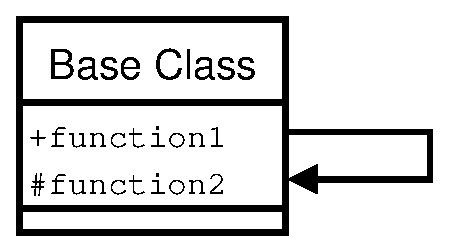
\includegraphics[width=4cm]{figures/base_class_only.eps}
\caption{A simple UML diagram of a base class with two member functions, where one calls the other.
\label{figure:baseonly}}
\end{center}
\end{figure}
%
If another class is created that inherits from the base class
then it could call one of the \public or \protected member functions
of the base class.  This could in turn call another member function
illustrated in figure~\ref{figure:nopolymorphism}.
%
\begin{figure}[h]
\begin{center}
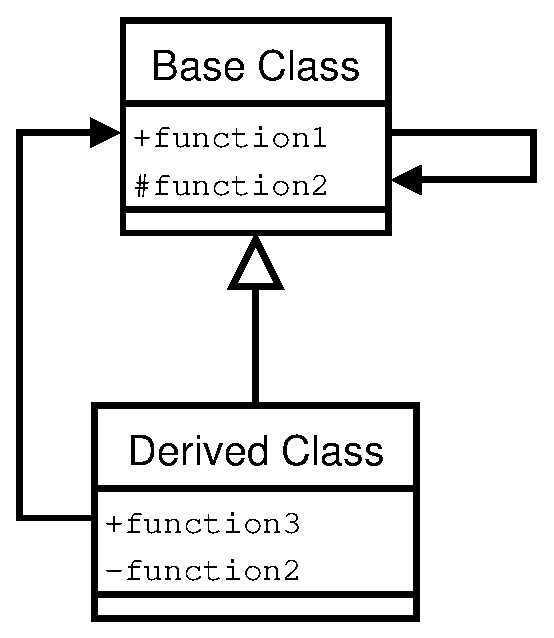
\includegraphics[width=5cm]{figures/no_polymorphism.eps}
\caption{A simple UML diagram of a derived class with two member functions, one of which calls a function in the base class which in turn calls another member function.
\label{figure:nopolymorphism}}
\end{center}
\end{figure}
%
Now consider that the derived class contains two member functions,
where one of which has the same name and parameter types as the member
function called by the base class.  If the derived class calls the
base class then without polymorphism the member function of the base
class calls the function within the base class.  Unsurprisingly the
base class method does not call the member function within the derived
class.

By introducing polymorphism it is possible to select which of the two
member functions is called: the one within the base class or the one
within the derived class.  It is therefore possible to write a program
that functions illustrated in figure~\ref{figure:polymorphism}.
%
\begin{figure}[h]
\begin{center}
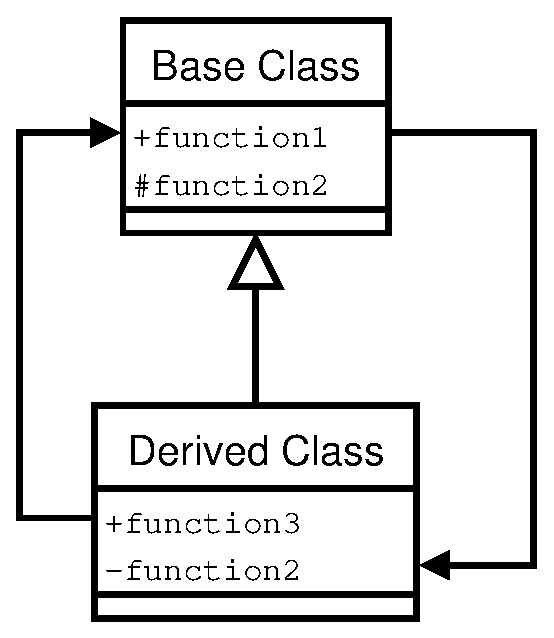
\includegraphics[width=5cm]{figures/polymorphism.eps}
\caption{A simple UML diagram of a derived class with two member functions, one of which calls a function in the base class which by polymorphism in turn calls a member function within the derived class.
\label{figure:polymorphism}}
\end{center}
\end{figure}
%
Implementations of programs illustrated in figures~\ref{figure:nopolymorphism}
and~\ref{figure:polymorphism} are given in example~11.

Within example~11 a base class \texttt{BasicParticle} and a derived
class \texttt{SmearedParticle} are implemented.  There are two forms
of the example code given: with polymorphism and without polymorphism.
There is only one difference between the two directories: in the
\texttt{with/} directory the method \texttt{calculateMass} is declared
as virtual void, where as in the \texttt{without/} directory the method is
simply declared as \texttt{void}.

\paragraph{Without Polymorphism}
In the \texttt{without/} directory the
\texttt{SmearedParticle} class inherits from the
\texttt{BasicParticle} base class.  In the \main function an instance
of the \texttt{SmearedParticle} class is created and the
\texttt{calculateMass} function is called by the
\texttt{assignFourVector} member function.  The value of the mass is
then printed.
%
\begin{verbatim}
int main() {
  double fourvector1[4] = {3.0, 4.0, 5.0, 7.35};
  ...
  SmearedParticle *smearedParticle = new SmearedParticle(fourvector1);
  ...
  cout << "smearedParticle mass = " << smearedParticle->getMass() <<  endl;
\end{verbatim}
%
The value returned from the \texttt{getMass} member function of the
\texttt{SmearedParticle} object is the same as that returned from the
one called from the \texttt{BasicParticle} object.  What is happening
is that the member function \texttt{assignFourVector} is calling the
\texttt{calculateMass} function within the \texttt{BasicParticle}
class and not the \texttt{SmearedParticle} class as required.  To get
around this problem polymorphism can be used.  

\paragraph{With Polymorphism}
In the \texttt{with/} directory the member function \texttt{calculateMass} is
defined as virtual within the header file \texttt{BasicParticle.hh}.
%
\begin{verbatim}
class BasicParticle {
...
protected:
...
  virtual void calculateMass();
};
\end{verbatim}
%
The effect of this is that when the \texttt{assignFourVector} member
function is called from the \texttt{BasicParticle} object then the
method \texttt{calculateMass} within the class \texttt{BasicParticle}
is called, but when the \texttt{assignFourVector} method is called via
the \texttt{SmearedParticle} class the method \texttt{calculateMass}
within the class \texttt{SmearedParticle} is called.

For polymorphism to work the member function in the base class must be
\texttt{virtual} and identical in its parameter types to the member
function declared in the derived class.  (It is good pratice to
declare the methods within the derived class that use polymorphism as
virtual too.)

%-----------------------------------------------------------------------------

\subsection{Interfaces}
Interfaces are abstract classes that contain only pure virtual
member functions.  A pure virtual member function is defined by
declaring a virtual member function to be equal to zero.  For instance,
in example~12 an interface containing a single pure virtual member function is
defined in the header file \texttt{IDataRecord.hh}:
%
\begin{verbatim}
class IDataRecord {
 public:
  virtual int appendRow(int *rowData) = 0;
};
\end{verbatim}
%
where \texttt{IDataRecord} is the class name of this interface.  Any
class that contains one or more pure virtual functions is defined as
being abstract and cannot be instantiated.  Furthermore any pure
virtual member function defined within a class should not implemented
within the class but rather must be implemented by a non-abstract
derived class.  Any class that is derived from an abstract class but
does not implement the inherited pure virtual functions will also be
an abstract class.  Notice therefore an interface can be used to
require a set of member functions to be present in a class that is
derived from it.

In example~12 classes \texttt{AsciiRecord} and \texttt{BinaryRecord}
inherit from the interface \texttt{IDataRecord}.  Both classes
\texttt{AsciiRecord} and \texttt{BinaryRecord} implement the pure
virtual member function of \texttt{IDataRecord} and are therefore not
abstract.  Again within this example the convention is used that the
derived classes implementation of the virtual function is declared as
virtual.  While this is not necessary for functionality it allows
anyone reading the code to quickly see which member functions are affected
by polymorphism.

When example~12 executes a pointer of \texttt{IDataRecord} type is
assigned the address of either a \texttt{AsciiRecord} or
\texttt{BinaryRecord} object.  As within the previous example the type
of object the pointer points to implies which virtual member function is
called.  Having created a pointer of \texttt{IDataRecord} type the
pointer is then passed to a function:
%
\begin{verbatim}
void fillRecord(IDataRecord *record) {
  int arr[] = {1,2,3,4,5,6,7,8,9,10};
  record->appendRow(arr);
}
\end{verbatim}
%
This function calls the member function \texttt{appendRow} defined within the
\texttt{IDataRecord} class.  Following polymorphism this method call
will actually call the \texttt{appendRow} method of \texttt{AsciiRecord} or
\texttt{BinaryRecord} depending on the type of object
\texttt{IDataRecord} points to.  The example therefore illustrates
that functions and classes can be written to perform operations on
interfaces rather than on every given class type within an inheritance
structure.

%-----------------------------------------------------------------------------

\subsection{Templates}
Templates can be used in conjunction with classes or functions.  Within
this course only class templates will be considered.  A
class template is a class where one or more parameters have a template
type.  In the case where similar functionality is needed to operate
over different types a templated class can be used to generate the
needed code.  Instead of writing several classes with different types within
the constructors and the member functions, one template can be
written.  For each usage of the class template the compiler generated
the needed extra class definitions.

Example~13 contains a simple class template called \texttt{Array}.
This class template contains an array of type \texttt{T}.  The type
\texttt{T} is determined when the template is instantiated and must be
one of those listed at the bottom of the
\texttt{Array.hh} header file.
\begin{verbatim}
template class Array<char>;
template class Array<int>;
template class Array<float>;
template class Array<double>;
\end{verbatim}
Within the \main function there are two instantiations of the
\texttt{Array} templated class.
\begin{verbatim}
int main() {
  ...
  Array<int> arrayInt(N);
  Array<double> arrayDouble(N);
  ...
\end{verbatim}
where the type \texttt{T} is given inside the \texttt{<>}
brackets.  Then in the code that follows the two methods
\texttt{setElement} and \texttt{getElement} are called from both
template generated objects.  The parameter types of these member
functions depends on the type specified in the instantiation.  The
files \texttt{Array.hh} and \texttt{Array.cc} demonstrate how to
declare and implement templated constructors, member functions and
data members of a class template.

%=======================================================================

\subsection{Problems}

\paragraph{Histogramming}
Starting from the files provided in the \texttt{problem\_04} directory,
complete the program by writing a class called \texttt{Histogram}.
Then follow the instructions in the \texttt{README} file to build and
test the final program.

\begin{itemize}
\item The \texttt{Histogram} class should include a constructor:
\begin{verbatim}
  Histogram(char *filename, int nbins, float min, float max);
\end{verbatim}
and two member functions:
\begin{verbatim}
  void saveHisto(void); // Save the histogram to file
  book(float value, float weight);  // Book an entry into the histogram.
\end{verbatim}
where \texttt{filename} is the output filename, \texttt{nbins} is the
number of bins, \texttt{min} and \texttt{max} are the limits,
\texttt{value} is the value to be booked and \texttt{weight} is the
weight to give the entry.

\item Create \texttt{private} data members to store the number of bins, the
entries in each bin, the limits of the histogram and the file name.

\item The \texttt{saveHisto} member function should write the contents
of the histogram to a text file, where each row of the file contains a
bin centre and then a number of entries.
\end{itemize}

\paragraph{Extended Array}
Starting from the files provided in the \texttt{problem\_05} directory,
complete the program by creating a class called
\texttt{DataContainer}.

\begin{itemize}
\item The \texttt{DataContainer} class should store an array and
its size as \texttt{private} data members:
\begin{verbatim}
  DATA_TYPE *m_array;
  int m_size;
\end{verbatim}
where \texttt{DATA\_TYPE} should be set via a \texttt{\#define}
statement in the class' header file:
\begin{verbatim}
#define DATA_TYPE float
\end{verbatim}

\item Provide a constructor of the form:
\begin{verbatim}
DataContainer::DataContainer(DATA_TYPE *array, int size)
{
  m_size = size;
  m_array = new DATA_TYPE[_size];
...
\end{verbatim}

\item Write member functions to perform arithmetic
operators for \texttt{*}, \texttt{+}, and \texttt{/}, which create a
new class containing array elements of the form:
\[z_i = x_i * y_i \:\:,\:\: z_i = x_i + y_i \:\:,\:\:  z_i = x_i /
y_i\]

\item Write a \texttt{printArray} member function to print the
contents of the \texttt{m\_array} private data member.
\end{itemize}

\paragraph{Inheritance}
Starting from the files provided in the \texttt{problem\_06} directory,
complete the program by writing three classes: \texttt{Particle},
\texttt{DetParticle} and \texttt{CalParticle}.

\begin{itemize}
\item Using inheritance, provide constructors of the form:
\begin{verbatim}
Particle (int id, double *p3vec);
DetParticle(int id, double *p3vec, int trackId);
CalParticle(int id, double mass, double *p3vec, double eCal);
\end{verbatim}
where \texttt{p3vec} is an array of three elements.

\item Store the data passed into each class in \texttt{private} data members.

\item Provide \texttt{public} member functions to access the data
members of each class.
\end{itemize}


\paragraph{Transformation Interface}
Starting from the files provided in the \texttt{problem\_07} directory,
complete the program by writing: (i) an interface class that has
member functions to perform a transformation and a reverse
transformation, (ii) a class implementation of the Transformation
interface to perform rotations in two dimensions.

\begin{itemize}
\item Create an interface class \texttt{ITranslation} that contains the virtual
member functions from \texttt{OffsetTranslation} as pure virtual functions.
\item Create a class called \texttt{RotationTranslation} that inherits from an
interface class \texttt{ITranslation}.
\begin{itemize}
\item Refer to OffsetTranslation for hints on
how \texttt{RotationTranslation} might be implemented.
\item A rotation in two dimensions can be calculated via:
\[ x' = x cos \theta - y sin \theta \]
\[ y' = y cos \theta + x sin \theta \]
where $\theta$ is the angle of rotation, $x$ is the original $x$ and
$x'$ is the rotated one.
\end{itemize}
\end{itemize}

\paragraph{Track Container}
Starting from the files provided in the \texttt{problem\_08} directory,
complete the program by writing a class template called
\texttt{TrackContainer}.   \texttt{TrackContainer} should allow
\texttt{float} and \texttt{double} template types to be instantiated.
The class should also contain public data members: $p_t$,
$\cos(\theta)$, $phi_0$, $d_0$ and $z_0$, where their type is set by
the template's instantiation.


%%%%%%%%%%%%%%%%%%%%%%%%%%%%%%%%%%%%%%%%%%%%%%%%%%%%%%%%%%%%%%%%%%%%%%%%

\section{The Standard Template Library \label{section:stl}}

The Standard Template Library (STL) contains templates which are:
containers, and algorithms to operate on these containers.  Within the
ISO/ANSI standard there are serveral containers:
%
\begin{center}
\begin{tabular}{|l|l|} \hline
Sequential Containers & $<$deque$>$ $<$list$>$ $<$queue$>$
$<$stack$>$ $<$vector$>$\\ \hline
Associative Containers & $<$map$>$ $<$set$>$ \\ \hline
\end{tabular}
\end{center}
%
In addition to these containers STL includes \texttt{numeric}
algorithms, generic \texttt{algorithm}s and \texttt{complex} class
templates.  The following subsections introduce
\texttt{complex}, \texttt{vector}, \texttt{list}, \texttt{iterators}
and \texttt{algorithms}.  More information on STL in general and areas
not covered in this course can be found in the recommended text books.

%-----------------------------------------------------------------------------

\subsection{Complex Numbers}
Complex numbers are implemented in a \texttt{complex} class.  
Example~14 introduces some of the \texttt{complex} operations available.  At
the top of the example~14 the \texttt{complex} header is included,
making the
\texttt{complex} classes and global methods accessible.
The allowed templated types for a complex number are:
\texttt{float}, \texttt{double}, and \texttt{long double}.  In the
example two of the three \texttt{complex} class types are implemented:
%
\begin{verbatim}
std::complex<float> complexFloat(3,4);
std::complex<double> complexDouble(-1,0);
\end{verbatim}
%
The \texttt{complex} class is part of the \texttt{std} namespace.
Therefore the class name must be used either with the \texttt{std::} specifier
explicitly or by quoting \texttt{using namespace std}.  The
constructor comes in three forms: including real and imaginary parts
as in the example, the copy constructor and the implicit default
constructor.  The type of the variables passed into the constructor
must match the type given in the template instantiation.  For example
\texttt{std::complex<float>} would mean that \texttt{complex(float,
float)} is the valid constructor.

After the instantiation of the \texttt{complex} objects the rest of
example~14 demonstrates some of the functionality available via the
inclusion of \texttt{<complex>}.

%-----------------------------------------------------------------------------

\subsection{Vectors}
For a physicist STL \texttt{vector}s are probably the most useful of
the STL container classes.  Basically a \texttt{vector} can be thought
of as an array with extra functionality.  Unlike an array
\texttt{vector}s do not have a fixed size and elements can be added
and removed as necessary.  Beyond this the class provides other
advanced functionality.  Example~15 demonstrates simple \texttt{vector}
usage.  Within the \main function one \texttt{vector} of \texttt{int}
type is created.
\begin{verbatim}
int main() {
  std::vector<int> intVector;
....
\end{verbatim}
Elements are then added to the vector using the \texttt{push\_back}
method.  As the vector increases in size the size is printed out.
Then the length of the vector is reduced by calling the member
function \texttt{pop\_back}, which pops elements off the end of the
vector.  Before the elements are popped off the back the value of the
element is printed retreived by calling the method \texttt{back}.

%-----------------------------------------------------------------------------

\subsection{Iterators}
Iterators provide access to the different elements of the data
container classes.  Iterators relate in a similar way to the container
classes as the pointer did to the array in
section~\ref{section:cppsyntax}.  For an iterator to step over the
correct amount of memory the iterator must be initialised from a data
container of the same type as it will be used with.  Iterators are
introduced in example~16.  Contained within this example a
\texttt{list} of \texttt{char} type is initialised with a string.
Then an iterator of the corresponding container type is created and
assigned with the address of the first element.
\begin{verbatim}
list<char>::iterator itr;
itr = charList.begin();
\end{verbatim}
Once the iterator has been initialised with the starting address it is
then used to iterate over all of the elements of the \texttt{list}.
The value of each element of the list is printed,
\begin{verbatim}
cout << *itr << " ";
\end{verbatim}
and the address stored in the iterator is moved on to the next element.
\begin{verbatim}
itr++;
\end{verbatim}

%-----------------------------------------------------------------------------

\subsection{Alogrithms}
STL provides a number of powerful algorithms which use iterators to
operate on data containers.  Example~17 introduces the sort algorithm.
Algorithm functionality is accessible via the inclusion of the header
file \texttt{<algorithm>}.  To use algorithms interators of type
according to the data container should be created.  Within example~17 a
vector of \texttt{int} type initialised with a random jumble of
numbers.  Two iterators of the same type are then created.
\begin{verbatim}
std::vector<int>::iterator first;
std::vector<int>::iterator last;
\end{verbatim}
These iterators are then assigned the memory addresses of the first and
last memory element of the vector.
\begin{verbatim}
first = numbers.begin();
last = numbers.end();
\end{verbatim}
The iterators are then passed to the sort algorithm.
\begin{verbatim}
std::sort(first,last);
\end{verbatim}
Since the algorithm methods are part of the \texttt{std} namespace the
specifier is used.  This is just one of the methods available.  Look
at one of the text books or in the header file for the other methods.

%-----------------------------------------------------------------------------

\subsection{Strings}
While many useful programs can be written with \texttt{cstring}s the
\texttt{string} class provides extra functionality and more
flexibility than a simple \texttt{cstring} character array.  The
\texttt{string} class is part of the Standard Template Library (STL)
and inherits many useful features from container base classes.  In
general terms the \texttt{string} class is a container which contains
an array of characters.  Unlike a \texttt{cstring} objects of the
\texttt{string} class have dynamic size and the memory allocated for
the storage of characters can be reduced or increased as needed.  Where
strings need to grow quickly it is also possible to allocate sections
of memory such that any appending operation does not necessarily
trigger additional memory operations.

Example~18 demonstrates some of the functionality of the
\texttt{string} class.  While this example implements many of the
\texttt{string} class member functions it does not use
\texttt{iterators}.  \texttt{iterators} are defined within the \texttt{string}
class and can be used in conjunction with some of its member functions
as well as the STL algorithms.

%-----------------------------------------------------------------------------

\subsection{String Streams}
A string stream is a stream connected to a \texttt{string} object.
Such a stream allows objects or simple variables to be inserted and
extracted from a string using stream syntax.  While C functions like
\texttt{sscanf} are still available within \cpp, string streams provide a
useful type safe means of converting variables to and from strings.
Example~19 demonstrates the type safe nature of the stream operators by
using an input string stream to convert a string into both an
\texttt{int} and a \texttt{double}.

%-----------------------------------------------------------------------------

\subsection{Stream Formatting}
When writing numbers into a stream it may be necessary to format the
numbers to have a particular precision or width.  Example~20
demonstrates some \cpp stream formatting options.  Again the advantage
of using \cpp streams over C functions like \texttt{printf} is that
\cpp streams are type safe.

%==============================================================================

\subsection{Problems}

\paragraph{Algorithms}
Create a vector object and fill it with sequential numbers from 0 to
100.  Then use the random\_shuffle algorithm to shuffle the elements.
\begin{verbatim}
  std::vector<int> numbers;
  ...
  first = numbers.begin();
  last = numbers.end();
  std::random_shuffle(first, last);
\end{verbatim}
Print the elements out before and after the random shuffling.  Then
find the position of the number 7 within the vector.

%%%%%%%%%%%%%%%%%%%%%%%%%%%%%%%%%%%%%%%%%%%%%%%%%%%%%%%%%%%%%%%%%%%%%%%%%%%%%%

\section{Particle Physics Applications \label{section:apps}}

%-----------------------------------------------------------------------------

\subsection{Interfacing with FORTRAN~77}

\cpp developers writing physics analysis programs may
want to access efficient and thoroughly tested FORTRAN algorithms.
Thankfully \cpp and FORTRAN~77 can be easily linked togther.  This
course discusses how to link FORTRAN~77 programs compiled with the
\texttt{gfortran} compiler together with \cpp programs compiled the
\texttt{g++} compiler.  While it may be possible to link to programs
compiled with other FORTRAN compilers it should be noted that the
symbols produced from other such compilers may well not follow the
rules given within this course.

Example~21 demonstrates all of the nuances of connecting FORTRAN~77 and
\cpp together.  This examples fills a FORTRAN common block using a
\cpp function, prints the contents of the common using a FORTRAN
function and then calls a FORTRAN function which in turn calls a \cpp
function.  The \texttt{main.cc} file includes \texttt{fortran.hh}.
This header file contains the declaration of an external struct
\texttt{forcom\_}, together with the
declaration of two functions implemented in FORTRAN
%
\begin{verbatim}
void commons_(void);
float call_back_(float *,char *, int);
\end{verbatim}
%
and a function implemented in \cpp
%
\begin{verbatim}
float mult_a__(float *);
\end{verbatim}
%
When example~21 executes the \texttt{fillCommon} function is called to
fill the FORTRAN common block \texttt{FORCOM} via the \cpp external
\texttt{struct} \texttt{forcom\_}.  The syntax for accessing the
\texttt{struct} data members is exactly the same as that used for accessing
public data members of an object.  The struct provides access to the
FORTRAN common because it has the same name within the compiled object
file and is declared to be external.  The \texttt{extern} prefix causes the
compiler not to define an additional memory block for the struct but
instead link the FORTRAN definition of the memory block to the \cpp
one.  Without the \texttt{extern} prefix the struct would occupy a
different memory location and therefore not provide access to the
FORTRAN common block.  While the mapping of the external struct to the
common block is possible via choosing the correct name it will not
function properly unless the order, type and size of the variables
declared in the struct match those declared in the FORTRAN common
block.  Notice however that the declaration of the \cpp struct is not
entirely the same as the FORTRAN common, for example:
%
\begin{verbatim}
int arr[2][3][4]
float farr[5][6]
\end{verbatim}
%
has the same memory mapping as
% 
\begin{verbatim}
INTEGER ARR(4,3,2)
REAL FARR(6,5)
\end{verbatim}
%
Notice that the outer array indices commute.  The last feature to
common block mapping is that FORTRAN strings do not contain string
terminators and therefore can contain a string as long as the number
of elements in the character array.

Once the common block has been filled the 
% 
\begin{verbatim}
commons_();
\end{verbatim}
%
function is called to print the values contained within the common
block.  The function 
% 
\begin{verbatim}
void commons_(void);
\end{verbatim}
%
is a declaration of the Fortan \texttt{SUBROUTINE}:
\begin{verbatim}
SUBROUTINE COMMONS
\end{verbatim}
When this \texttt{SUBROUTINE} is compiled the \texttt{gfortran} compiler
creates an object containing a symbol of the form:
\begin{verbatim}
void commons_(void);
\end{verbatim}
%
The next thing the \main function does is to call
% 
\begin{verbatim}
call_back_(&a,name,size);
\end{verbatim}
%
which is a call to the FORTRAN \texttt{FUNCTION}
\begin{verbatim}
FUNCTION CALL_BACK(A,NAME)
\end{verbatim}
which in turn calls
%
\begin{verbatim}
C = MULT_A(A)
\end{verbatim}
%
which is in fact a \cpp function
\begin{verbatim}
float mult_a_(float *a) {
  return (*a)*10.;
}
\end{verbatim}
FORTRAN~77 uses pointers implicitly but when FORTRAN functions are
called from \cpp these pointers must be declared explicitly.  While the
FORTRAN programmer is not aware of it the \texttt{gfortran} compiler
compiles in an extra integer for each string in a SUBROUTINE or
FUNCTION call.  The purpose of this extra integer is to store the
length of the FORTRAN string.  For example
%
\begin{verbatim}
SUBROUTINE STRINGS(A, B, C)
IMPLICIT NONE
CHARACTER*(*) A, B, C
...
\end{verbatim}
%
becomes
\begin{verbatim}
void strings_(char *a, char *b, char *c, 
              int size_a, int size_b, int size_c);
\end{verbatim}

%-----------------------------------------------------------------------------

\subsection{HepMC and HepPDT}

When most particle physics programs were written in FORTRAN~77 most
generators provided an event record in the \texttt{HEPEVT} common
block format.  Most modern experiments now use \cpp,
HepMC~\cite{hepmc} for their event records, and HepPDT~\cite{heppdt}
for their particle data.  Example~22 and 25 demonstrate some
applications of HepMC and example~25 introduces HepPDT.

\paragraph{$\pi^0$ decay generator}

Example~22 demonstrates the use of the \texttt{HepMC} package for
storing the event record of a $\pi^0$ decay generator.  The \main
function creates a new event container, generatates a $\pi^0$
particle, decays the $\pi^0$ into two photons, and finally prints the
event record to the screen.  The source code for this program is
divided up into: \texttt{MonteCarlo} - containing two static methods
to generate a $\pi^0$ particle and produce a two body generic decay;
\texttt{LorentzBoost} - a wrapper class providing a static method to
lorentz boost a fourvector via the FORTRAN code contained in
\texttt{lorentz.for}.  When the program runs all of the event data are
recorded within the event record \texttt{GenEvent}.  Once the
\texttt{GenEvent} instance has been created
\texttt{GenVertex}s can be added.  Each
\texttt{GenVertex} can connect a number of different
\texttt{GenParticle}s together.  


The \main function instantiates a \texttt{GenEvent} object and then
calls a static member function of the \texttt{MonteCarlo} class:
%
\begin{verbatim}
HepMC::GenParticle pi0 = MonteCarlo::generate();
\end{verbatim}
%
to create a \texttt{GenParticle} that describes a $\pi^0$
particle.  The \main function then calls a second static member
function of the \texttt{MonteCarlo} class:
%
\begin{verbatim}
MonteCarlo::twoBody(evt,&pi0,22,22,0.,0.);
\end{verbatim}
%
to produce a decay of the $\pi^0$ into two photons.  The
\texttt{twoBody} member function starts by creating a vertex and then
adds the $\pi^0$ particle to it
%
\begin{verbatim}
HepMC::GenVertex *vert = new HepMC::GenVertex();
vert->add_particle_in(parent);
\end{verbatim}
%
Once the two daughter photons have been produced they are also added
to this vertex,
%
\begin{verbatim}
vert->add_particle_out(new HepMC::GenParticle(fvecDaughter1,
                                              particleId1,1));
vert->add_particle_out(new HepMC::GenParticle(fvecDaughter2,
                                              particleId2,1));
\end{verbatim}
%
and the vertex is then added to the \texttt{GenEvent} event container:
%
\begin{verbatim}
evt->add_vertex(vert);
\end{verbatim}
%
The complete decay is then printed in the \main function.

%-----------------------------------------------------------------------------

\subsection{ROOT}

ROOT~\cite{rootweb} is a data analysis package written in \cpp and
supported at CERN.  Tutorials and how-tos and other documentation can
be downloaded from the ROOT web site~\cite{rootweb}.  This course
focuses on introducing basic features of ROOT needed for a data
analysis.

\paragraph{Histograms}
When analysing large statistical samples histograms provide an
important means of visualising accumulated results.  Example~23 uses
ROOT to produce a single one dimensional histogram.  Within the \main
function memory associated with root histograms is initialised,
\begin{verbatim}
TROOT simple("histos","Histogram Examples");
\end{verbatim}
the root file that will contain the histogram is opened, writing
over any existing file of the same name by quoting \texttt{"RECREATE"},
\begin{verbatim}
TFile *rfile = new TFile(argv[1],"RECREATE","Histogram Example");
\end{verbatim}
a one dimension histogram is then created,
\begin{verbatim}
TH1F *histo = new TH1F("histo","Sine Wave",nbinsx,xlow,xup);
\end{verbatim}
the histogram is filled,
\begin{verbatim}
histo->Fill(x,w);
\end{verbatim}
then the contents of the root memory including the single one
dimensional histogram is written to the ROOT file.
\begin{verbatim}
rfile->Write();
\end{verbatim}  

\paragraph{TTrees}
\texttt{TTree}s are flexible data containers.  Each \texttt{TTree}
can have several \texttt{TBranches}.  Data are written in rows to all
\texttt{TBranch}es of a \texttt{TTree}, but can be read back from a
single \texttt{TBranch} or all the attached \texttt{TBranch}es at once.

Basic \texttt{TTree} IO and plotting macros are introduced in
example~24.  The example provides two options: (i) write a
\texttt{TFile} called \texttt{tree.root} containing the TTree, or (ii)
read the \texttt{TTree} back and print values stored in it.  When the program writes the \texttt{TTree} the
\begin{verbatim}
void writeTree(char *filename)
\end{verbatim}
function is called.  This function opens a new \texttt{TFile}
\begin{verbatim}
TFile *root_file = TFile::Open(filename,"RECREATE");
\end{verbatim}
and checks to see if the file is open.  In ROOT the last file that was
opened becomes the present working directory and therefore associated with the following \texttt{TTree} instantiation
\begin{verbatim}
TTree *tree = new TTree("tree","test tree");
\end{verbatim}
where the key \texttt{``tree''} has to be unique and the title \texttt{``test tree''} does not.

Once a \texttt{TTree} has been instantiated \texttt{TBranch}es can be added to it.
\begin{verbatim}
tree->Branch("Run",&run,"Run/I");
tree->Branch("Event",&event,"Event/I");
tree->Branch("x",&x,"x/F");
tree->Branch("y",&y,"y/F");
tree->Branch("z",&z,"z/F");
\end{verbatim}
Each of these member function calls
causes a new \texttt{TBranch} to be instantiated and connected to the
parent \texttt{TTree} object.  The arguments of the \texttt{Branch} member
function are: the key, the address of an associated variable and the
label.  When the \texttt{TTree} member function 
%
\begin{verbatim}
tree->Fill();
\end{verbatim}
%
is called the value in the memory at the address assigned to each
\texttt{TBranch} is saved into the \texttt{TTree}.  Finally when all
the data have been entered into the \texttt{TTree} the \texttt{TFile}
is saved,
% 
\begin{verbatim}
root_file->Write();
\end{verbatim}
%
flushing any remaining data to disk.

The \texttt{readTree} function reads a \texttt{TTree} from a
\texttt{TFile} and prints out each entry from all the \texttt{TBranch}es.  The \texttt{TFile} is opened and then a pointer to
the \texttt{TTree} is collected by supplying the key name of the
\texttt{TTree}
%
\begin{verbatim}
Tree *tree = (TTree*)root_file->Get("tree");
\end{verbatim}
%
where a cast to a \texttt{TTree*} is necessary because the
\texttt{Get} member function of \texttt{TFile}, (inherited from
\texttt{TDirectory}), returns type \texttt{TObject*}.  After
collecting a pointer to the \texttt{TTree}, a pointer to each
\texttt{TBranch} is collected
%
\begin{verbatim}
TBranch *run_branch = tree->GetBranch("Run");
\end{verbatim}
%
and the branches addresses are set to be addresses of variables defined within
the scope of the \texttt{readTree} function
%
\begin{verbatim}
run_branch->SetAddress(&run);
\end{verbatim}
%
Instead of reading each \texttt{TBranch} individually data from the
\texttt{TTree} are copied on mass into the \texttt{TBranch} addresses
by calling
%
\begin{verbatim}
tree->GetEvent(i); 
\end{verbatim}
If it is necessary to read data from just one \texttt{TBranch} the
\texttt{GetEvent} member function of that branch can be called.

Once the program has been compiled and run the macro \texttt{plot.C}
can be used to plot some of the content of the \texttt{TTree}:
\begin{verbatim}
src]$ root
root [0] .x ../macros/plot.C("plot.ps");
root [1] .q
\end{verbatim} %$
The macro creates another ROOT file containing a single histogram.
This can be plotted from the command line:
\begin{verbatim}
src]$ root -l histos.root
root [1] _file0->ls();                                            
TFile**         histos.root     Analysis Histograms
 TFile*         histos.root     Analysis Histograms
  KEY: TH2F     h2;1    x:y {y<20}
root [2] h2->Draw();
root [3] .q
\end{verbatim} %$
In the \texttt{plot.C} macro it is not possible to use the Write
member function of the TFile class to write this histogram to the
TFile because this only writes files from the present working
directory to the TFile.  It is possible to write ROOT macros which are
not functions but these are not subject to the same error checking
standard and are therefore often buggy.

\paragraph{Putting it all together}
Example~25 is the most complicated example of the course and
demonstrates some uses of HepMC, HepPDT, ROOT, and interfacing with
FORTRAN.  The example is composed of two programs:
\texttt{TruthNtuple} and \texttt{Analysis}.  \texttt{TruthNtuple} uses 
the PYTHIA event generator to fill a TTree with event records from
inelastic non-diffractive p-p interactions at 10TeV.  To do this
\texttt{TruthNtuple} calls PYTHIA to generate an event, and copy the
result into the \texttt{HEPEVT} common block.  Then HepMC is used to
copy the \texttt{HEPEVT} common block into a \texttt{GenEvent} record.
The \texttt{GenEvent} record is then copied into a set of vectors
which are in turn stored in the \texttt{TTree}.  To enable ROOT
storage of these STL containers the ROOT dictionaries have to be
created.  This is simply done by creating the ROOT dictionaries from
the LinkDef.h file.

Once \texttt{TruthNtuple} has been run the \texttt{Analysis} program
can be run to read the data back.  This program reads all of the
events and prints the contents of the 7th event to the standard
output.  The data members associated with the \texttt{TTree} are part
of the \texttt{Tree\_McTruth} class and were copied from a
\texttt{MakeClass($\;$)} call:
\begin{verbatim}
src]$ root pythia.root
root [0] mctree->MakeClass();
root [1] .q
\end{verbatim} %$
The version from the \texttt{MakeClass($\;$)} call was then adapted to
check if the \texttt{TBranch} was present in the \texttt{TTree}.  From
the data stored in the \texttt{TTree} some other useful quantities
such as the pseudorapidity, transverse momentum and the mass of the
particles are calculated.

%=============================================================================

\subsection{Problems}

\paragraph{B Mesons from PYTHIA}
Starting from the files provided in the \texttt{problem\_10} directory
complete program by writing a class called \texttt{HepevtTree} to
store all data from the \texttt{HEPEVT} common block in a TTree.

\paragraph{Minimum Bias Physics}
Take example 25 and histrogram the number of charged particles per
unit of pseudorapidity and per unit of transverse momentum.  Implement
these histograms in the \texttt{Analysis} program.  Then use a ROOT
macro to plot the histograms to ps files.

\bibliographystyle{plain}
\bibliography{HepCppIntroGuide}

\end{document}
